\documentclass{article}
\usepackage[utf8]{inputenc}
\usepackage{hyperref}
\usepackage[letterpaper, portrait, margin=1in]{geometry}
\usepackage{enumitem}
\usepackage{amsmath}
\usepackage{amsthm}
\usepackage{booktabs}
\usepackage{graphicx}
\usepackage{float}
\usepackage{hyperref}
\usepackage[flushleft]{threeparttable}
\usepackage{textcomp}
\hypersetup{
colorlinks=true,
    linkcolor=black,
    filecolor=black,      
    urlcolor=blue,
    citecolor=black,
}
\usepackage{natbib}

\usepackage{titlesec}
\bibliographystyle{chicago}
\newcommand{\bib}{references.bib}

\newcommand\iid{\stackrel{\mathclap{iid}}{\sim}}
\newcommand\asym{\stackrel{\mathclap{a}}{\sim}}
\newcommand\convprob{\xrightarrow{p}}
\newcommand\convdist{\xrightarrow{d}}
\newcommand{\N}{\mathbb{N}}
\newcommand{\Z}{\mathbb{Z}}
\newcommand{\E}{\text{E}}
\newcommand{\V}{\text{Var}}
\newcommand{\Av}{\text{Avar}}
\newcommand{\se}{\text{se}}
\newcommand{\corr}{\text{Corr}}
\newcommand{\cov}{\text{Cov}}
\newcommand{\norm}{\text{Normal}}
\newcommand{\indep}{\perp \!\!\! \perp}

\begin{document}
% The tex content below is similar to the given main.tex
 
\title{Homework 3}
\author{Environmental Economics II\\
Maghfira Ramadhani}
\date{\today}
\maketitle

In this assignment, we are given imaginary data on an energy-efficiency retrofit program in Atlanta. The research hypothesis is whether the program reduced energy use. The experiment done in such way that after recruiting the households for the program, we assigned them to treatment and control groups. Treatment homes received the retrofits on the first of the month and control homes did not have any work done.

\begin{enumerate}
\item Suppose that for for a home $i$, the underlying relationship between electricity use and predictor variable is given by 
\begin{align}
    y_i=e^\alpha\delta^{d_i}z_i^{\gamma}e^{\eta_i} \label{h3e1}
\end{align}

where $y_i$ is the electricity use, $e$ is Euler's number or the base of the natural logarithm, $d_i$ is a binary variable equal to one if home $i$ received the retrofit program, $z_i$ is a vector of the other control variables, and $\eta_i$ is unobserved error, and $\{\alpha,\delta,\gamma\}$ are the parameter to estimates.


\begin{enumerate}
    \item Show that $\ln(y_i)=\alpha+\ln(\delta)d_i+\gamma\ln(z_i)+\eta_i$
    \\\textbf{Answer}\\
    Rewrite equation \eqref{h3e1} by taking natural log on both sides and distribute the natural log on the right hand side of the equation, we have
    \begin{align}
         \ln(y_i)&=\ln\left(e^\alpha\delta^{d_i}z_i^{\gamma}e^{\eta_i}\right) \notag\\
        \Leftrightarrow\ln(y_i)&=\ln(e^\alpha)+\ln(\delta^{d_i})+\ln(z_i^{\gamma})+\ln(e^{\eta_i}) \notag\\
        \Leftrightarrow\ln(y_i)&=\alpha+\ln(\delta^{d_i})+\gamma\ln(z_i)+\eta_i \notag\\
        \Leftrightarrow\ln(y_i)&=\alpha+\ln(\delta)d_i+\gamma\ln(z_i)+\eta_i\label{h3e2}.
    \end{align}\qed
    \item What is the intuitive interpretation of $\delta$?
    \\\textbf{Answer}\\
    Let's take the expectation of Equation \eqref{h3e1} conditional on $d_i$, we have
    \begin{align}
        \E[y_i|d_i=1,z_i]&=e^\alpha\delta z_i^{\gamma}e^{\eta_i}\\
        \E[y_i|d_i=0,z_i]&=e^\alpha z_i^{\gamma}e^{\eta_i}
    \end{align}
    Dividing the first equation by the second equation, we have
    \begin{align}
        \delta=\frac{\E[y_i|d_i=1,z_i]}{\E[y_i|d_i=0,z_i]} \label{h3e5} 
    \end{align}
    which means $\delta$ translates to the ratio of the expected electricity use of the treated house to the expected electricity use of the nontreated house conditional on other control variables. The intuitive interpretation of $\delta$ related to the context of the program is as follows. If the program improve the energy efficiency of the house, then the electricity use of the treatment group will be lower than the control group, and $\delta$ will be less than one. If the program does not improve the energy efficiency of the house, then the electricity use of the treatment group will be higher than the control group, and $\delta$ will be greater than one. If the program does not have any effect on the energy efficiency of the house, then the electricity use of the treatment group will be the same as the control group, and $\delta$ will be equal to one.
    \item Show that $\frac{\Delta y_i}{\Delta d_i}=\frac{\delta-1}{\delta^{d_i}}y_i$. What is the intuitive interpretation of $\frac{\Delta y_i}{\Delta d_i}$?
    \\\textbf{Answer}\\
    Note that since $d_i$ is a binary variable, the average marginal effect of $d_i$ is the difference in the expected value of $y_i$ between the treatment and control group, i.e:
    \[\frac{\Delta y_i}{\Delta d_i}=\E[y_i|d_i=1,z_i]-\E[y_i|d_i=0,z_i].\]
    By using previous result in equation \eqref{h3e5}, we have 
    \begin{align}
        \E[y_i|d_i=1,z_i]-\E[y_i|d_i=0,z_i]&=\delta\E[y_i|d_i=0,z_i]-\E[y_i|d_i=0,z_i]=(\delta-1)\E[y_i|d_i=0,z_i] \label{h3e6}
    \end{align}
    Since we only observed $y_i$ from the data we need to know what exactly is $\E[y_i|d_i=0]$. Since the relationship between $y_i$ and $d_i$ is non-linear, it might be useful to apply potential outcome framework with equation \eqref{h3e2}. Suppose $y_{0i}$ is the potential outcome of $y_i$ if $d_i=0$ and $y_{1i}$ is the potential outcome of $y_{1i}$ if $d_i=1$ conditional on $z_i$. From the underlying relationship, note that for every house $i$, we have $y_{1i}/y_{0i}=\delta$. Applying the potential outcome framework, we have
    \begin{align}
        \ln(y_i)=\ln(y_{0i})+[\ln(y_{1i})-\ln(y_{0i})]d_i
        \Leftrightarrow& \ln\left(\frac{y_i}{y_{0i}}\right)=d_i\ln\left(\frac{y_{1i}}{y_{0i}}\right)=d_i\ln(\delta) \notag\\
        \Leftrightarrow& \frac{y_i}{y_{0i}}=e^{d_i\ln(\delta)}=\delta^{d_i} \notag\\
        \Leftrightarrow& y_{0i}=\frac{1}{\delta^{d_i}}y_i \label{h3e7}
    \end{align}
    Substituting equation \eqref{h3e7} to \eqref{h3e6}, we can obtain the average marginal effect of $d_i$ as follows:
    \[\frac{\Delta y_i}{\Delta d_i}=\E[y_i|d_i=1,z_i]-\E[y_i|d_i=0,z_i]=\frac{\delta-1}{\delta^{d_i}}y_i.\]\qed

    The intuitive interpretation of $\frac{\Delta y_i}{\Delta d_i}$ is the reduction in monthly electricity consumption in kWh if a house received a retrofit.
    \item Show that $\frac{\delta y_i}{\delta z_i}=\gamma\frac{y_i}{z_i}$. What is the intuitive interpretation of $\frac{\delta y_i}{\delta z_i}$ when $z_i$ is the size of the home in square feet?
    \\\textbf{Answer}\\
    Since $z_i$ is a vector of control variables, we can apply the chain rule to equation \eqref{h3e2} with respect to $z_i$ as follows:
    \begin{align}
        \frac{\partial \ln(y_i)}{\partial z_i}=\frac{\partial \ln(y_i)}{\partial y_i}\frac{\partial y_i}{\partial z_i}=\frac{1}{y_i}\frac{\partial y_i}{\partial z_i}=\frac{\gamma}{z_i}\Rightarrow \frac{\partial y_i}{\partial z_i}=\gamma\frac{y_i}{z_i} \label{h3e8}
    \end{align}\qed

    If $z_i$ is the size of the home in square feet, then the intuitive interpretation of $\frac{\delta y_i}{\delta z_i}$ is the change in monthly electricity consumption in kWh if the size of the home in square feet increase by one square feet. We can expect the sign of $\gamma$ to be positive. The larger the size of the home, the more electricity it consumes.

    \item Estimate the log-transformed equation via OLS on the transformed parameters. Save the coefficient estimates and the average marginal effects estimates of $z_i$ and $d_i$ $\left(\frac{\delta y_i}{\delta z_i}\text{ and }\frac{\Delta y_i}{\Delta d_i}\right)$. Bootstrap the 95\% confidence intervals of the coefficient estimates and the marginal effects estimates using 1000 sampling replications. Display the results in a table with three columns (one for the variable name, one for the coefficient estimates, and once for the marginal effect estimate). Show the 95\% confidence intervals for each estimate under each number.
    \\\textbf{Answer}\\
    \begin{table}[H]\centering
        \begin{threeparttable}
            \caption{Parameter and average marginal effect estimates from Python}
            \label{t1:estimates}
            \begin{tabular}{lccc}
\toprule
{} & Parameter estimates & Average marginal effects estimates \\
\midrule
Constant                                    &              -0.769 &                                    \\
                                            &     [-1.804, 0.292] &                                    \\
=1 if home received retrofit                &               0.904 &                           -113.975 \\
                                            &      [0.893, 0.916] &                [-129.003, -99.489] \\
Square feet of home                         &               0.894 &                              0.629 \\
                                            &      [0.879, 0.908] &                      [0.616, 0.64] \\
Outdoor average temperature (\textdegree F) &               0.281 &                              3.997 \\
                                            &      [0.038, 0.522] &                     [0.554, 7.454] \\
Observations                                &                1000 &                               1000 \\
\bottomrule
\end{tabular}

            \begin{tablenotes}
            \small \item Column 1 shows the estimates of $\alpha,\delta,\gamma_{sqft}$, and $\gamma_T$ parameter and their 95\% confidence intervals. Column 2 shows the average marginal effect estimates of the retrofit ($\frac{\Delta y_i}{\Delta d_i}$), square feet of home ($\frac{\delta y_i}{\delta sqft_i}$), and outdoor temperature ($\frac{\delta y_i}{\delta T_i}$) and their 95\% confidence intervals.
            \end{tablenotes}
        \end{threeparttable}
        \end{table}

        \begin{table}[H]\centering
            \begin{threeparttable}
                \caption{Parameter and average marginal effect estimates from Stata}
                \label{t2:estimates}
                \begin{tabular}{l*{2}{c}}
\hline\hline
                    &\multicolumn{1}{c}{Parameter Estimates}&\multicolumn{1}{c}{AME Estimates}\\
\hline
Constant            &      -0.769&            \\
                    &[-1.848,0.310]&            \\
=1 if home received retrofit&       0.904&    -110.729\\
                    &[0.893,0.916]&[-130.589,-90.869]\\
Square feet of home &       0.894&       0.622\\
                    &[0.880,0.909]&[0.607,0.638]\\
Outdoor average temperature (\textdegree F)&       0.281&       2.851\\
                    &[0.039,0.524]&[-2.057,7.758]\\
\hline
Observations        &       1,000&       1,000\\
\hline\hline
\end{tabular}

                \begin{tablenotes}
                \small \item Column 1 shows the estimates of $\alpha,\delta,\gamma_{sqft}$, and $\gamma_T$ parameter and their 95\% confidence intervals. Column 2 shows the average marginal effect estimates of the retrofit ($\frac{\Delta y_i}{\Delta d_i}$), square feet of home ($\frac{\delta y_i}{\delta sqft_i}$), and outdoor temperature ($\frac{\delta y_i}{\delta T_i}$) and their 95\% confidence intervals.
                \end{tablenotes}
            \end{threeparttable}
            \end{table}
    
    The difference between Stata and Python result for AME estimates is very likely due to difference in the bootstrap sample randomization. Even if I set the seed in Stata and numpy the same, the realization is difference.
    \item Graph the \textbf{average marginal effects} of outdoor temperature and square feet of home with bands for their bootstrapped confidence intervals so that they are easy to interpret and compare.
    \\\textbf{Answer}\\
    \begin{figure}[H]
        \centering
        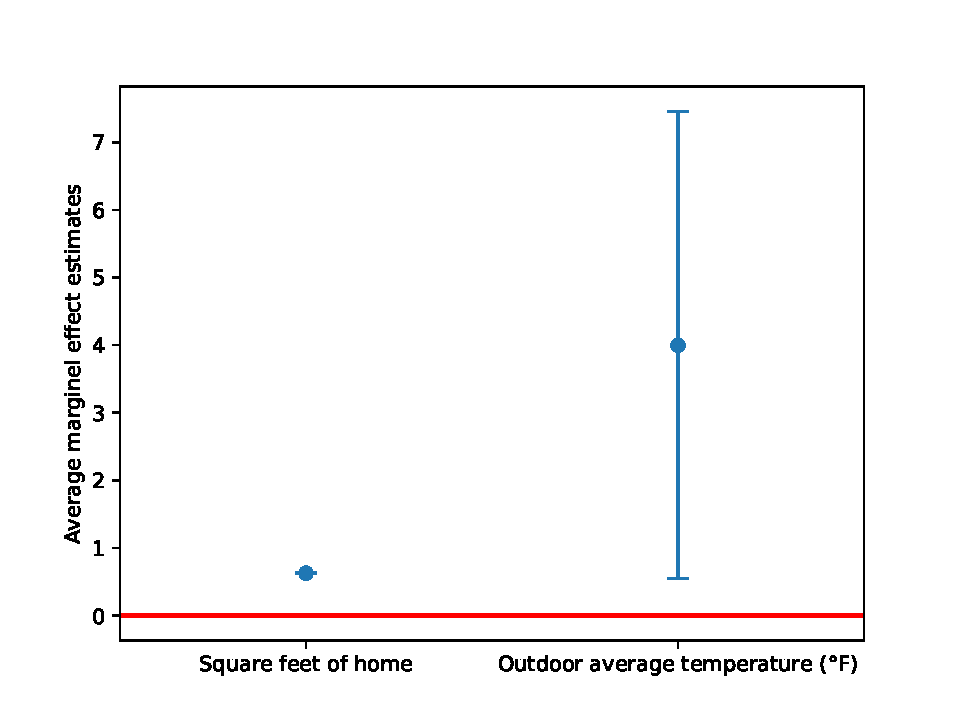
\includegraphics[scale = 0.7]{./figure/ame.pdf}
        \caption{Average marginal effect estimates of outdoor temperature and square feet of home from Python}
        \label{f1:ame}
    \end{figure}
    The interpretation of the estimates in Figure \ref{f1:ame} is as follows. The larger the house size, the more electricity it consumes with an average additional consumption of around 0.6 kWh per additional square feet. Similarly, the higher the outdoor temperature, the more electricity a house consumes with the increase ranges from 0.5 to 7.4 kWh per one \textdegree F of increase.
\end{enumerate}


\end{enumerate}
\end{document}